% !TEX program = xelatex
% 策联杯 A 题参赛论文半成品（无目录；第 1 页为摘要专用页）
% 编译：xelatex -> bibtex -> xelatex -> xelatex
% 请勿在全文任何位置填写姓名、学校或队号。
\documentclass[a4paper,12pt,UTF8,zihao=-4]{ctexart}

\usepackage{geometry}
\geometry{a4paper,left=2.5cm,right=2.5cm,top=2.5cm,bottom=2.5cm}
\usepackage{amsmath,amssymb,bm}
\usepackage{booktabs,tabularx,longtable,multirow,makecell}
\usepackage{graphicx}
\usepackage{xcolor}
\usepackage{caption}
\usepackage{subcaption}
\usepackage{setspace}
\usepackage{enumitem}
\usepackage{hyperref}
\usepackage{fancyhdr}
\usepackage{titlesec}
\usepackage{array}
\usepackage{threeparttable}
\usepackage{listings}
\usepackage{tcolorbox}
\usepackage{placeins}
\usepackage{cite}

\hypersetup{
  colorlinks=true,
  linkcolor=black,
  citecolor=black,
  urlcolor=blue
}

\graphicspath{{figures/}{../output/A/}}

% 页码：页脚居中，阿拉伯数字从 1 连续编号（摘要页即为第 1 页）
\pagestyle{fancy}
\fancyhf{}
\renewcommand{\headrulewidth}{0pt}
\fancyfoot[C]{\thepage}
\fancypagestyle{plain}{%
  \fancyhf{}%
  \renewcommand{\headrulewidth}{0pt}%
  \fancyfoot[C]{\thepage}%
}

\captionsetup{font=small,labelsep=quad}
\setlist[itemize]{leftmargin=2em,itemsep=0.2em,topsep=0.3em}
\setlist[enumerate]{leftmargin=2em,itemsep=0.2em,topsep=0.3em}
\setstretch{1.25}

\lstset{
  basicstyle=\small\ttfamily,
  breaklines=true,
  columns=fullflexible,
  frame=single,
  numbers=left,
  numberstyle=\tiny\color{gray},
  keywordstyle=\color{blue!70!black},
  commentstyle=\color{green!50!black},
  stringstyle=\color{red!60!black},
  showstringspaces=false,
  tabsize=4,
  xleftmargin=1.2em,
  framexleftmargin=1.2em
}
\newtcolorbox{todobox}[1][]{
  colback=yellow!8,
  colframe=orange!70!black,
  fonttitle=\bfseries,
  title={待完成 / 框架占位},
  #1
}

\newtcolorbox{resultbox}[1][]{
  colback=blue!4,
  colframe=blue!50!black,
  fonttitle=\bfseries,
  title={已完成结果（仓库现有成果）},
  #1
}

\title{锂离子电池快充策略对寿命衰减的影响建模与优化}
\author{} % 按赛制不得出现参赛者信息
\date{}

\begin{document}

% ============================================================
% 第一页：摘要专用页（含标题和关键词，无需英文）
% ============================================================
\thispagestyle{plain}
\begin{center}
{\heiti\zihao{3} 锂离子电池快充策略对寿命衰减的影响建模与优化}
\end{center}
\vspace{0.8em}

\noindent{\heiti\zihao{4} 摘\quad 要}

\vspace{0.4em}
\noindent
提高充电倍率可缩短补能时间，但过高电流会加速容量衰减。本文基于 MIT--Stanford 公开的 49 块 A123 18650 型磷酸铁锂电池循环老化数据，围绕两阶段快充策略 \(C_1\)--\(Q_1\)--\(C_2\)，研究快充参数对寿命衰减的影响，并讨论寿命预测与策略优化问题。

针对问题一，本文对循环数据进行逐电池、逐字段的 IQR 异常检测与前后邻域均值填补，共替换 559 个异常单元格；提取 9 种快充策略，并以第 200 次循环的 SOH 作为观测窗口内的寿命代理指标（数据尚未覆盖 \(\mathrm{SOH}=80\%\) 的真实寿命终止）。在 40 块满 200 圈电池中，SOH 均值为 0.9914，按 25\%/75\% 分位数划分得到长寿命 10 块、中等寿命 20 块、短寿命 10 块。策略层面，寿命最长为 \(3.6\mathrm{C}(80\%)-3.6\mathrm{C}\)，寿命最短为 \(3.7\mathrm{C}(31\%)-5.9\mathrm{C}\)（NEWSTRUCTURE）。同名义参数但带/不带 NEWSTRUCTURE 标签的策略寿命差异明显，提示批次或实验结构不可忽略。

针对问题二，本文以 \(\mathrm{SOH}_{200}\) 和 200 圈衰减量为寿命代理指标，在同一实验结构的 34 块完整样本上完成策略间 Kruskal--Wallis 检验、参数关联/稳健回归诊断与 SOH 纵向混合效应分析。策略间总体差异显著（\(H=12.3346, p=0.0305\)），但 Holm 校正后未识别出显著的单一策略对；参数共线性较强，故结果仅作样本内关联解释。

针对问题三，拟利用截至第 150 次循环的早期数据，提取健康特征并建立 SOH 衰减预测模型，预报第 151--200 次循环 SOH，并外推至 \(\mathrm{SOH}=80\%\) 的循环寿命；同时比较不同早期窗口长度及策略信息的作用。\textcolor{gray}{（本节定量结果待补全）}

针对问题四，拟建立充电时间模型与寿命衰减模型，在已有实验策略及其合理邻域内进行充电时间--寿命的多目标权衡，给出推荐策略并讨论外推风险。\textcolor{gray}{（本节定量结果待补全）}

\vspace{0.8em}
\noindent{\heiti 关键词：}锂离子电池；快充策略；SOH；循环寿命；IQR；寿命预测；多目标优化

\clearpage

% ============================================================
% 第二页起：正文（不要目录）
% ============================================================
\section{问题重述}

随着新能源汽车与储能系统对补能效率的要求提高，锂离子电池快充成为缩短充电时间的主要手段。然而较高充电电流会增强极化、加剧热效应并加速副反应，从而加快容量衰减、缩短循环寿命\cite{severson2019datadriven,liu2019fastcharging,ahmed2017enabling}。电池健康状态定义为
\begin{equation}
\mathrm{SOH}=\frac{Q_{\mathrm{current}}}{Q_{\mathrm{initial}}},
\label{eq:soh}
\end{equation}
本题以 \(\mathrm{SOH}=80\%\) 作为寿命终止（EOL）判定阈值。

本题充电过程采用两阶段快充：以倍率 \(C_1\) 从 \(0\%\) SOC 充至切换点 \(Q_1\)，再以倍率 \(C_2\) 从 \(Q_1\) 充至 \(80\%\) SOC，随后以 1C 恒流--恒压（CC-CV）补至满电，至电流降至 \(C/50\) 结束。各电池放电条件一致，主要差异在充电策略。数据来自 MIT--Stanford 公开循环老化实验\cite{severson2019datadriven,matrdataset}，包含 49 块额定容量 1.1\,Ah 的 A123 18650 磷酸铁锂电池。

需要完成的研究任务为：
\begin{enumerate}[label=\textbf{问题\arabic*.}]
  \item 整理数据，提取策略、充电时间、SOH 变化与循环寿命信息，分析寿命分布并解释典型长/短寿命策略差异。
  \item 分析策略参数 \(C_1,Q_1,C_2\) 对循环寿命的影响及其统计显著性与可能机制。
  \item 基于截至第 150 次循环的数据预测第 151--200 次循环 SOH，并外推 EOL 循环寿命。
  \item 兼顾充电时间与寿命衰减，在实验策略及其合理邻域内优化快充策略。
\end{enumerate}

\section{问题分析与总体思路}

问题一属于探索性数据分析：在尚未达到真实 EOL 的观测窗口内，需要定义可比较的寿命代理指标，并完成清洗、可视化与典型策略提取。问题二强调参数非正交，不宜按完全析因实验解释因果关系。问题三是早期循环预测与外推。问题四是充电时间与衰减率的多目标决策。四问递进关系为：数据整理 \(\rightarrow\) 影响分析 \(\rightarrow\) 寿命预测 \(\rightarrow\) 策略优化。

\begin{todobox}
问题三至问题四的模型推导、数值表与最终推荐策略尚未写入仓库，下文相应小节仅给出可直接填充的结构、符号与拟采用方法，待后续结果补入后删除本框并替换为正式论述。
\end{todobox}

\section{符号说明与基本假设}

\subsection{主要符号}
\begin{table}[htbp]
\centering
\caption{主要符号说明}
\label{tab:notation}
\begin{tabular}{cl}
\toprule
符号 & 含义 \\
\midrule
\(\mathrm{SOH}\) & 电池健康状态，见式\eqref{eq:soh} \\
\(C_1,C_2\) & 第一、二阶段充电倍率（C-rate） \\
\(Q_1\) & 阶段切换 SOC（\%） \\
\(N\) & 循环次数 \\
\(N_{\mathrm{EOL}}\) & \(\mathrm{SOH}=80\%\) 对应的循环寿命 \\
\(\mathrm{SOH}_{200}\) & 第 200 次循环的 SOH（寿命代理） \\
\(T_{\mathrm{charge}}\) & 平均充电时间（min） \\
\bottomrule
\end{tabular}
\end{table}

\subsection{基本假设}
\begin{enumerate}
  \item 各电池放电协议一致，寿命差异主要由充电策略及电池个体差异引起。
  \item 在 200 次循环窗口内未达到 \(\mathrm{SOH}=80\%\)，故问题一以 \(\mathrm{SOH}_{200}\) 作为寿命代理指标，并在文中明确其与真实循环寿命的区别。
  \item 带 \(\mathrm{NEWSTRUCTURE}\) 后缀的策略与同名无后缀策略视为不同实验结构/批次标签，分析时不合并。
  \item IQR 筛出的离群点视为统计异常而非已证实的传感器故障，清洗仅用于本题指定分析。
  \item 问题四若扩展连续参数，取值限制在已有实验数据的凸包或合理邻域内，避免无约束外推。
\end{enumerate}

\section{问题一：数据整理与快充策略对寿命影响的初步分析}

\subsection{数据来源与结构}

本题使用赛题提供的 MIT--Stanford 锂离子电池循环老化数据\cite{severson2019datadriven,matrdataset}。\texttt{battery\_summary.csv} 记录 49 块电池的策略参数 \(C_1,Q_1,C_2\)、初始容量、平均充电时间、平均内阻、平均温度及问题三测试标记 \texttt{prediction\_test}；\texttt{cycle\_train.csv} 记录逐循环的容量、SOH、平滑 SOH、充电时间、内阻与平均温度，共 9350 行。非测试电池记录至第 200 次循环，9 块测试电池仅至第 150 次循环。输入质量检查表明：\texttt{battery\_id}+\texttt{cycle} 无重复；循环表无缺失；汇总表有 3 个缺失单元格，其中 \(C_1\) 的结构性缺失予以保留，不参与循环数据清洗。最大循环数分布为 \(\{150:9,\,200:40\}\)。

\subsection{寿命指标定义}

题设循环寿命为 \(\mathrm{SOH}\) 降至 \(80\%\) 时的循环次数 \(N_{\mathrm{EOL}}\)。本数据集在 200 次循环内 \(\mathrm{SOH}_{200}\) 范围为 \(0.9497\sim 1.0002\)，均值 \(0.9914\)，\textbf{尚未覆盖真实寿命终止}。因此问题一采用
\begin{equation}
\mathrm{LifeProxy}_i=\mathrm{SOH}_{i}(N=200)
\label{eq:lifeproxy}
\end{equation}
作为观测窗口内的使用寿命代理：该值越高，表示前 200 圈健康保持越好。后文箱线图、分布图与策略标签均基于该代理指标。若需与问题三衔接，可进一步计算衰减率
\begin{equation}
\mathrm{FadeRate}_i=\frac{\mathrm{SOH}_i(1)-\mathrm{SOH}_i(N)}{N-1},
\label{eq:fade}
\end{equation}
并在问题二、三中统一使用。\cite{severson2019datadriven,plett2015bms1}

\subsection{IQR 清洗}

对每块电池、每个测量字段（capacity、SOH、SOH\_smooth、chargetime、IR、Tavg）分别计算下、上四分位数 \(Q_1,Q_3\) 及四分位距 \(\mathrm{IQR}=Q_3-Q_1\)。将
\[
x\notin\bigl[Q_1-1.5\,\mathrm{IQR},\; Q_3+1.5\,\mathrm{IQR}\bigr]
\]
的观测标为异常，并用同一电池、同一字段中距离最近的前后正常值均值替换；若仅有单侧邻域则用该侧值。共替换 559 个单元格，分字段数量为：capacity 36、SOH 36、SOH\_smooth 17、IR 142、Tavg 142、chargetime 186。原始 \texttt{data/} 文件未改写，清洗结果保存为 \texttt{output/A/cycle\_train\_cleaned.csv}。

\subsection{策略提取与 200 圈样本}

由汇总表提取 49 块电池的 \texttt{battery\_id}--\texttt{policy} 对照，得到 9 种策略（表~\ref{tab:policy_extract} 给出示意，完整表见支撑材料 \texttt{charge\_policy.csv}）。寿命统计分析仅纳入最大循环数恰为 200 的 40 块电池，排除 9 块问题三测试电池，以免 150 圈终点与 200 圈终点混比。

\begin{table}[htbp]
\centering
\caption{部分电池快充策略提取结果（完整 49 行见支撑材料）}
\label{tab:policy_extract}
\begin{tabular}{cl}
\toprule
battery\_id & policy \\
\midrule
1 & \texttt{3\_6C-80PER\_3\_6C} \\
4 & \texttt{80PER\_3\_6C} \\
7 & \texttt{4\_8C\_80PER\_4\_8C} \\
10 & \texttt{5C\_67PER\_4C\_NEWSTRUCTURE} \\
16 & \texttt{3\_7C\_31PER\_5\_9C\_NEWSTRUCTURE} \\
49 & \texttt{4\_8C\_80PER\_4\_8C\_NEWSTRUCTURE} \\
\bottomrule
\end{tabular}
\end{table}

\subsection{SOH 变化曲线}

以 1 号电池为例绘制清洗后 SOH 与平滑 SOH 随循环次数的变化，见图~\ref{fig:soh1}。早期循环中 SOH 可略高于 1（容量活化/测量波动），随后缓慢下降。该图用于展示单电池衰减形态，策略间对比见后文分布图与箱线图。

\begin{figure}[htbp]
\centering
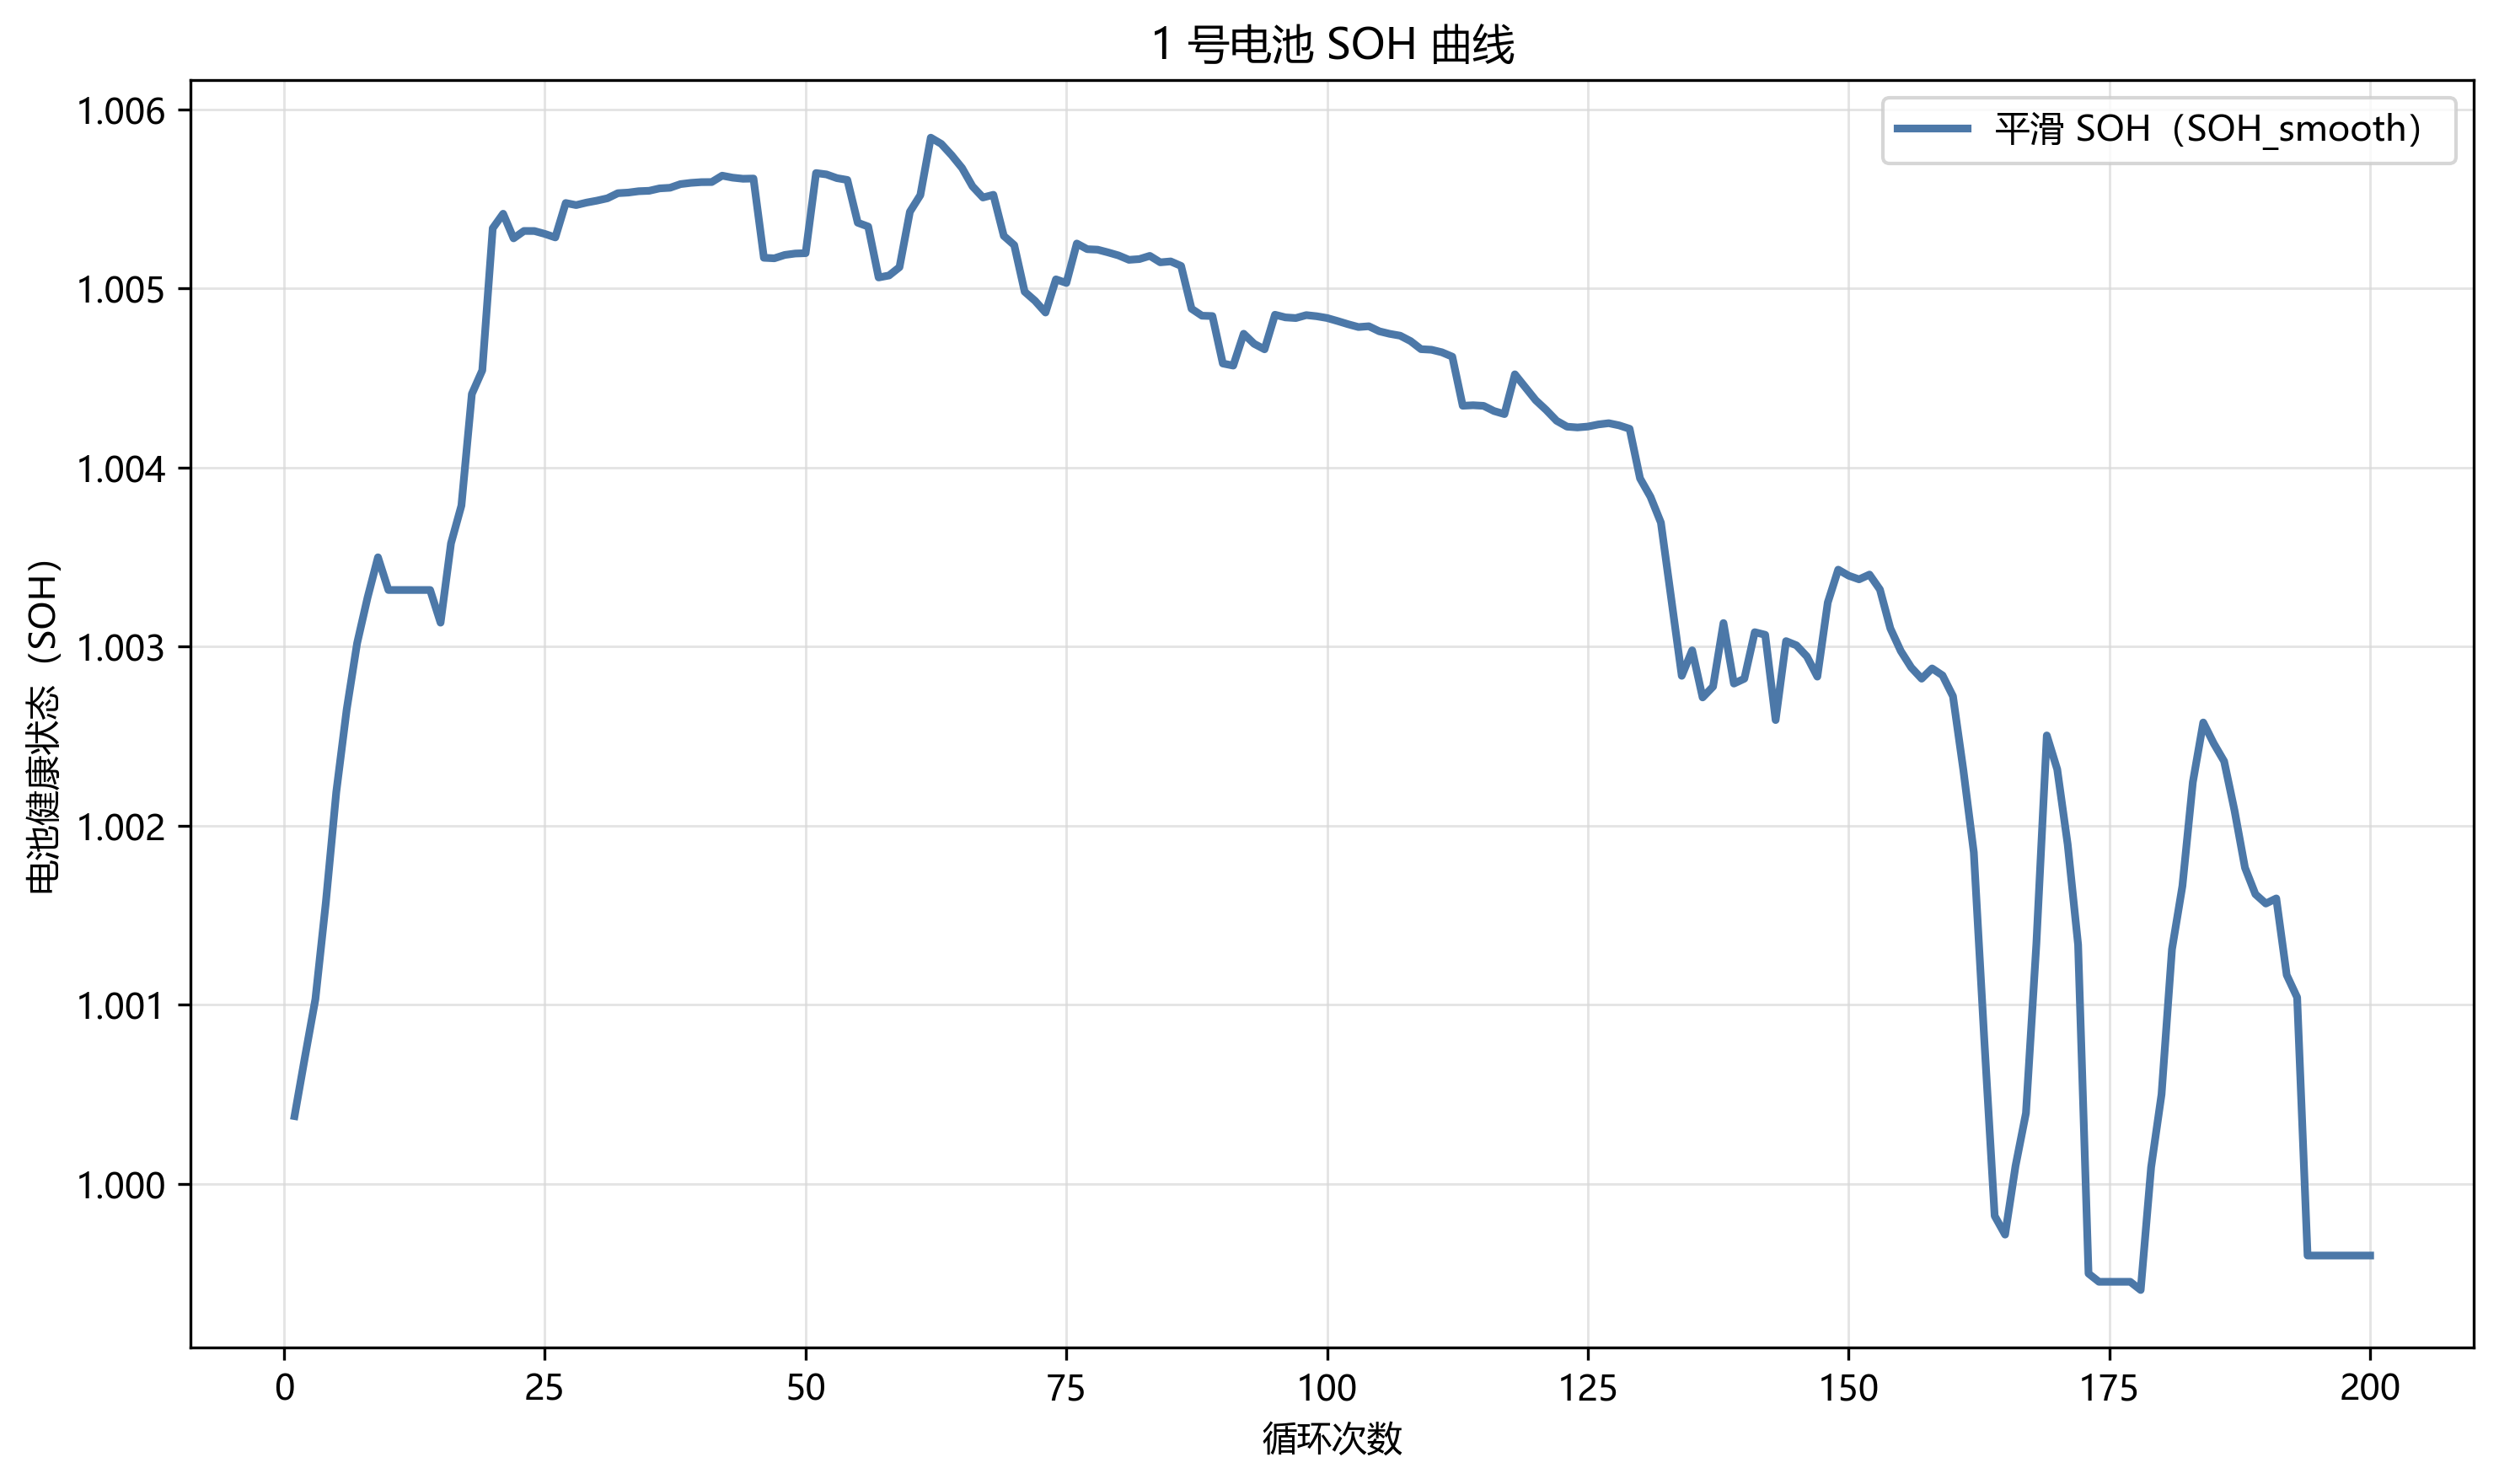
\includegraphics[width=0.88\textwidth]{SOH_1_example.png}
\caption{1 号电池 SOH 曲线（清洗后原始 SOH 与平滑 SOH）}
\label{fig:soh1}
\end{figure}

\subsection{寿命分布统计分析}

对 40 块电池的 \(\mathrm{SOH}_{200}\) 绘制直方图。取样本 75\% 分位数
\[
\mathrm{critical\_SOH_{high}}=0.996103
\]
为长寿命分界（红色虚线），25\% 分位数
\[
\mathrm{critical\_SOH_{low}}=0.993433
\]
为短寿命分界（蓝色虚线）。据此分类：长寿命 10 块、中等寿命 20 块、短寿命 10 块。分布见图~\ref{fig:sohhist}。

\begin{figure}[htbp]
\centering

\includegraphics[width=0.88\textwidth]{SOH_summary.png}
\caption{第 200 次循环 SOH 分布及长/短寿命分位数分界线}
\label{fig:sohhist}
\end{figure}

\(\mathrm{SOH}_{200}\) 与平均充电时间的散点图见图~\ref{fig:scatter}，按策略着色。可见充电时间较短的策略并不一律对应更低 SOH，时间--寿命关系并非简单单调，为问题四的多目标权衡提供现象基础。

\begin{figure}[htbp]
\centering

\includegraphics[width=0.92\textwidth]{SOH_chargetime.png}
\caption{第 200 次循环 SOH 与平均充电时间散点图（按策略着色）}
\label{fig:scatter}
\end{figure}

不同策略下 \(\mathrm{SOH}_{200}\) 的箱线图见图~\ref{fig:box}，并叠加上述两条分界线。各策略汇总统计见表~\ref{tab:policy_summary}。

\begin{figure}[htbp]
\centering

\includegraphics[width=0.98\textwidth]{charge_policy.png}
\caption{不同充电策略下第 200 次循环 SOH 箱线图}
\label{fig:box}
\end{figure}

\begin{table}[htbp]
\centering
\small
\caption{各充电策略第 200 次循环 SOH 与充电时间汇总（仅 200 圈样本）}
\label{tab:policy_summary}
\begin{threeparttable}
\begin{tabular}{lcccccc}
\toprule
策略 & \(n\) & SOH 中位数 & SOH 范围 & 充电时间范围/min & 标签 \\
\midrule
\texttt{3\_6C-80PER\_3\_6C} & 2 & 0.9977 & 0.9952--1.0002 & 13.378--13.386 & 长寿命 \\
\texttt{4\_8C\_80PER\_4\_8C\_NEWSTRUCTURE} & 5 & 0.9963 & 0.9497--0.9970 & 11.038--11.038 & 长寿命 \\
\texttt{5C\_67PER\_4C\_NEWSTRUCTURE} & 6 & 0.9952 & 0.9948--0.9966 & 10.042--10.044 & 中等 \\
\texttt{5\_3C\_54PER\_4C\_NEWSTRUCTURE} & 7 & 0.9954 & 0.9938--0.9974 & 10.042--10.044 & 中等 \\
\texttt{5\_6C\_36PER\_4\_3C\_NEWSTRUCTURE} & 7 & 0.9941 & 0.9930--0.9968 & 10.041--10.045 & 中等 \\
\texttt{5\_6C\_19PER\_4\_6C\_NEWSTRUCTURE} & 7 & 0.9939 & 0.9933--0.9953 & 10.042--10.044 & 中等 \\
\texttt{4\_8C\_80PER\_4\_8C} & 2 & 0.9854 & 0.9814--0.9894 & 10.058--10.068 & 短寿命 \\
\texttt{80PER\_3\_6C} & 2 & 0.9805 & 0.9679--0.9930 & 13.376--13.388 & 短寿命 \\
\texttt{3\_7C\_31PER\_5\_9C\_NEWSTRUCTURE} & 2 & 0.9658 & 0.9601--0.9715 & 10.111--10.156 & 短寿命 \\
\bottomrule
\end{tabular}
\begin{tablenotes}
\footnotesize
\item 注：策略类型按策略内 SOH 中位数与总体 25\%/75\% 分位阈值比较得到。\(n\) 为满 200 圈电池数。
\end{tablenotes}
\end{threeparttable}
\end{table}

\subsection{典型长寿命与短寿命策略}

入选规则：以策略内 \(\mathrm{SOH}_{200}\) 中位数为序；长寿命要求中位数 \(\ge 0.996103\)，短寿命要求中位数 \(\le 0.993433\)。

\textbf{寿命最长策略：}\texttt{3\_6C-80PER\_3\_6C}，中位数 \(0.997734\)，范围 \(0.995232\)--\(1.000235\)，平均充电时间约 \(13.38\)\,min（\(n=2\)）。

\textbf{典型长寿命策略：}\texttt{4\_8C\_80PER\_4\_8C\_NEWSTRUCTURE}，中位数 \(0.996334\)，但范围宽至 \(0.949733\)--\(0.996955\)，含一个明显偏低个体，解读时需结合离散程度。

\textbf{寿命最短策略：}\texttt{3\_7C\_31PER\_5\_9C\_NEWSTRUCTURE}，中位数 \(0.965818\)，范围 \(0.960114\)--\(0.971521\)，\(C_2=5.9\mathrm{C}\) 为全样本最高第二阶段倍率。

\textbf{典型短寿命策略：}\texttt{80PER\_3\_6C} 与 \texttt{4\_8C\_80PER\_4\_8C}。

\subsection{长、短寿命策略差异的初步解释}

结合两阶段快充物理图像\cite{liu2019fastcharging,dubarry2009lfp,ma2024mcc}，可将差异归纳如下。

\begin{enumerate}
  \item \textbf{高 SOC 区间高倍率。} 最短寿命策略在 \(Q_1=31\%\) 之后仍以 \(5.9\mathrm{C}\) 充电至 \(80\%\) SOC。中高 SOC 下浓差极化、锂沉积风险与产热更显著，与题干“高 SOC 区间继续高倍率可能加剧老化”一致。
  \item \textbf{低倍率、高 \(Q_1\) 并不自动等于长寿命。} \texttt{80PER\_3\_6C} 充电时间长达约 \(13.4\)\,min，但 \(\mathrm{SOH}_{200}\) 仍偏低，说明“充得慢”不是充分保护条件，可能与长时间处于中高 SOC 或批次差异有关。
  \item \textbf{同名义参数、不同标签不可等同。} \texttt{4\_8C\_80PER\_4\_8C} 与 \texttt{4\_8C\_80PER\_4\_8C\_NEWSTRUCTURE} 的 \(C_1,Q_1,C_2\) 相同，但前者被标为短寿命、后者中位数落入长寿命。二者平均充电时间分别约为 \(10.06\)\,min 与 \(11.04\)\,min，说明实际过程或批次并不相同。\texttt{NEWSTRUCTURE} 应理解为后期实验框架标签，\textbf{不是}“充电条件完全相同”。
  \item \textbf{样本与窗口局限。} 若干策略仅 2 块满 200 圈电池；早期三策略与 NEWSTRUCTURE 策略跨批次对比应降级为现象观察。正式因果推断与显著性检验留待问题二\cite{kutner2005applied,jes2024fastchargevariability}。
\end{enumerate}

\begin{todobox}
问题一仍可补充：（1）策略参数总表（每策略 \(C_1,Q_1,C_2\) 与 IR、温度均值）；（2）NEWSTRUCTURE 内部单独排序作为公平对比主结论；（3）9 策略平均 SOH--cycle 曲线。上述不影响已给出的清洗、分布与典型策略结论。
\end{todobox}

\FloatBarrier

\section{问题二：充电策略及其参数对寿命衰减的影响}

\begin{todobox}
本节为建模框架。仓库中尚无问题二的专用脚本与统计表。补全后应删除本框，填入检验统计量、回归系数与诊断图。
\end{todobox}

\subsection{问题分析}

问题一已表明策略间 \(\mathrm{SOH}_{200}\) 存在可见差异，但 \(C_1,Q_1,C_2\) 并非完全独立变化，策略数仅 9、部分组 \(n=2\)。因此本节重点是：组间差异是否具有统计显著性；三参数与寿命的相关/回归关系；不同 SOC 区间高倍率是否对应不同衰减特征；以及机制解释的局限性\cite{ruiz2023degradation,wang2024agingmodels,geslin2023joule}。

\subsection{数据与可比性规则（拟采用）}

\begin{enumerate}
  \item 主分析：满 200 圈样本；因变量优先用 \(\mathrm{SOH}_{200}\) 或 \(\mathrm{FadeRate}\)。
  \item 公平对比：NEWSTRUCTURE 内部互比作为主结论；带/不带该标签的同参数策略不作同条件重复实验。
  \item 若纳入测试电池，统一截断至第 150 圈再比较，避免窗口不一致。
\end{enumerate}

\subsection{模型一：策略间差异的显著性检验}

将策略视为分组因子。若各组近似正态且方差齐，采用单因素 ANOVA；否则采用 Kruskal--Wallis 检验，事后比较用 Tukey HSD 或 Dunn 检验，并报告效应量 \(\eta^2\)\cite{kutner2005applied}。

\textbf{待填结果：} \(H\) 或 \(F\) 统计量、\(p\) 值、两两比较中显著的策略对。

\subsection{模型二：参数与寿命的回归 / 相关分析}

考察
\begin{equation}
\mathrm{LifeProxy}_i=\beta_0+\beta_1 C_{1,i}+\beta_2 Q_{1,i}+\beta_3 C_{2,i}+\beta_4 C_{2,i}\cdot \mathbf{1}\{Q_{1,i}<Q^\ast\}+\varepsilon_i.
\label{eq:reg}
\end{equation}
因参数共线，可同时报告 Spearman 相关、方差膨胀因子（VIF），必要时采用混合效应（策略随机截距）\cite{pinheiro2000mixed}。交互项用于刻画“高倍率发生在低/高 SOC 区间”的差异。

\textbf{待填结果：} 系数表、标准化系数或变量重要性、残差诊断。

\subsection{不同 SOC 区间高倍率的衰减特征}

将充电过程拆为低 SOC 段 \([0,Q_1]\) 与高 SOC 段 \([Q_1,80\%]\)，比较 \(C_1\) 主导段与 \(C_2\) 主导段对 \(\mathrm{FadeRate}\) 的边际贡献。预期：在数据允许时，\(C_2\) 对寿命的负向作用强于同等幅度的 \(C_1\)\cite{liu2019fastcharging,ma2024mcc}。

\subsection{机制讨论与局限}

拟从 SEI 生长、锂沉积、极化与产热等 LFP 相关路径讨论\cite{dubarry2009lfp,dubarry2012alawa,li2026degradation}，并明确：策略非正交、早期衰减幅度小、cell-to-cell 变异与批次标签会限制因果识别。

\section{问题三：基于早期循环的电池寿命预测}

\begin{todobox}
本节为建模框架。9 块测试电池已在 \texttt{battery\_summary.csv} 中由 \texttt{prediction\_test}=1 标记，循环数据截至第 150 圈。预测表、误差指标与 EOL 外推结果待补入。
\end{todobox}

\subsection{问题分析}

实际中往往只能获得前期循环，无法等待完整老化。本题要求：用截至第 150 次循环的数据预测第 151--200 次循环 SOH，并进一步估计 \(\mathrm{SOH}=80\%\) 的循环寿命；同时比较不同早期窗口长度，讨论策略信息与早期衰减特征的作用\cite{severson2019datadriven,attia2021statistical,geslin2023joule,zhang2018lstm,zhang2019boxcoxmc}。

\subsection{特征提取（拟采用）}

\begin{table}[htbp]
\centering
\caption{问题三拟提取的特征类别}
\label{tab:feat}
\begin{tabular}{ll}
\toprule
类别 & 示例 \\
\midrule
策略参数 & \(C_1,Q_1,C_2\) 及策略编码 \\
衰减趋势 & 前 \(k\) 圈 SOH 斜率、曲率、幂律/指数拟合参数 \\
过程量 & 充电时间、IR、温度的均值与变化率 \\
分段差 & \(\Delta\mathrm{SOH}_{1\rightarrow 50}\)、\(\Delta\mathrm{SOH}_{50\rightarrow 100}\)、\(\Delta\mathrm{SOH}_{100\rightarrow 150}\) \\
\bottomrule
\end{tabular}
\end{table}

优先使用 \texttt{SOH\_smooth}。若后续引入放电电压曲线类特征 \(\Delta Q(V)\)，需回源完整公开数据\cite{attia2021statistical,matrdataset}。

\subsection{预测模型（拟采用）}

\textbf{经验衰减模型}（可解释）：
\begin{equation}
\mathrm{SOH}(n)=1-a\,n^{b}\quad\text{或}\quad \mathrm{SOH}(n)=a\mathrm{e}^{-bn}+c,
\label{eq:emp}
\end{equation}
用 1--150 圈拟合，外推 151--200 及 \(N_{\mathrm{EOL}}\)。

\textbf{统计 / 机器学习模型：} 以早期统计特征预测后续 SOH 或衰减率，候选包括正则化线性模型、随机森林 / XGBoost、高斯过程；序列模型可试 LSTM\cite{zhang2018lstm}。验证建议：在 40 块非测试电池上做“截断 150 圈 \(\rightarrow\) 预测 151--200”的交叉验证，再对 9 块测试电池给出最终预报，避免同策略信息泄漏。

\subsection{评价指标与窗口比较}

对 151--200 圈报告 RMSE、MAE 与 \(R^2\)；对 \(N_{\mathrm{EOL}}\) 报告外推圈数。比较输入窗口 \(k\in\{50,100,150\}\) 的精度差异。消融：有/无 \((C_1,Q_1,C_2)\)。

\textbf{待填：} 9 块测试电池的 SOH 预测曲线、误差表、EOL 点估计。

\section{问题四：兼顾充电时间与寿命衰减的策略优化}

\begin{todobox}
本节为建模框架。优化应优先在已有 9 种实验策略内比较；若连续优化，参数须限制在实验数据合理邻域并说明依据\cite{attia2020closedloop,plett2022bms3,frazier2018bo,deb2001moea}。
\end{todobox}

\subsection{决策变量与目标}

决策变量 \(x=(C_1,Q_1,C_2)\)。目标为在较短充电时间下降低衰减速率或延长寿命：
\begin{equation}
\min_{x}\; F(x)=\begin{bmatrix} T_{\mathrm{charge}}(x)\\ \mathrm{DecayRate}(x)\end{bmatrix}
\quad\text{或}\quad
\min_{x}\; w_1 T_{\mathrm{charge}}(x)+w_2\,\mathrm{DecayRate}(x).
\label{eq:moo}
\end{equation}

\subsection{充电时间模型（拟采用）}

分段恒流近似
\begin{equation}
T_{\mathrm{charge}}\approx \frac{Q_1}{C_1}+\frac{0.8-Q_1}{C_2}+T_{\mathrm{CV}},
\label{eq:time}
\end{equation}
并用 \texttt{mean\_chargetime} 回归校准。问题一散点图已显示充电时间与策略分组相关，可用于检验该近似。

\subsection{寿命衰减模型}

沿用问题二回归或问题三预测模型，得到 \(\mathrm{DecayRate}(x)\) 或 \(\mathrm{SOH}_{200}(x)\)。在已有策略上先做离散 Pareto 比较，再考虑邻域连续搜索。

\subsection{约束与邻域}

建议参数盒约束取自样本极值（以最终校核为准）：\(C_1\in[3.6,5.6]\)，\(Q_1\in[19,80]\)，\(C_2\in[3.6,5.9]\)。超出实验凸包的组合须标明外推风险。

\subsection{推荐策略与对比（待填）}

给出推荐 \((C_1^\ast,Q_1^\ast,C_2^\ast)\)，并与问题一的典型长寿命策略 \texttt{3\_6C-80PER\_3\_6C}、\texttt{4\_8C\_80PER\_4\_8C\_NEWSTRUCTURE} 及短寿命策略 \texttt{3\_7C\_31PER\_5\_9C\_NEWSTRUCTURE} 对比充电时间与寿命代理。说明适用范围（LFP、两阶段快充、早期循环窗口）与不可外推情形。


\section{结论与展望}

\begin{resultbox}
\textbf{问题一已形成的结论：}
\begin{itemize}
  \item 循环数据经 IQR 清洗后可用于策略对比；原始数据文件未改写。
  \item 在满 200 圈的 40 块电池中，第 200 次循环 SOH 均值为 0.9914，尚未达到 80\% EOL。
  \item 按策略内 SOH 中位数，最长寿命策略为 \(3.6\mathrm{C}(80\%)-3.6\mathrm{C}\)，最短为 \(3.7\mathrm{C}(31\%)-5.9\mathrm{C}\)（NEWSTRUCTURE）。
  \item 高 SOC 区间维持高 \(C_2\) 的策略更容易出现更快衰减；同参数不同标签策略不可直接等同。
\end{itemize}
\end{resultbox}

\begin{resultbox}
\textbf{问题二结论：}
\begin{itemize}
  \item 在同一实验结构的 34 块完整样本上，六种策略的 \(\mathrm{SOH}_{200}\) 分布存在总体差异（Kruskal--Wallis：\(H=12.3346,p=0.0305\)）。
  \item Holm 校正后的两两比较均未显著，故不对具体策略作确定性的优劣排序。
  \item \(Q_1\) 与 200 圈衰减量呈显著负 Spearman 相关，但 \(C_1\)、\(C_2\) 共线性严重；参数效应仅解释为样本内关联。
\end{itemize}
\end{resultbox}

\begin{todobox}
补充问题三预测精度与 EOL 估计、问题四推荐策略及与长短寿命策略的对比；讨论模型局限与可推广范围。
\end{todobox}

\section*{参考文献}
\bibliographystyle{unsrt}
\bibliography{refs}

% ============================================================
% 附录（页数不限）
% ============================================================
\appendix
\section{支撑材料文件列表}

按赛制，支撑材料单独打包为压缩文件（RAR/ZIP，不超过 20\,MB），本附录列出其内容。本次提交的压缩包为 \texttt{A20260700.rar}，其根目录包含：LaTeX 工程（\texttt{main.tex}、\texttt{refs.bib}、\texttt{sections/}）、论文图件（\texttt{figures/}）、可运行源代码（\texttt{src/}）与赛制要求的 AI 使用说明（\texttt{关于AI的使用说明.pdf}）。赛题原始数据 \texttt{data/battery\_summary.csv}、\texttt{data/cycle\_train.csv} 不作为“自主查阅数据”重复提交，但建模程序依赖它们运行。

\begin{table}[htbp]
\centering
\caption{支撑材料包含的文件}
\label{tab:support}
\small
\begin{tabular}{p{0.42\textwidth}p{0.48\textwidth}}
\toprule
路径 & 说明 \\
\midrule
\texttt{main.tex} & 支撑材料 LaTeX 主文档（四题正文与全部附录） \\
\texttt{refs.bib} & 参考文献库（与论文引用一一对应） \\
\texttt{关于AI的使用说明.pdf} & 赛制要求的 AI 工具使用说明（工具、环节、提示方式、采纳与核验） \\
\texttt{figures/question1/} & 问题一图件（5 张 PNG） \\
\texttt{figures/question2/} & 问题二图件（6 张 PNG） \\
\texttt{figures/question3/} & 问题三图件（9 张 PNG） \\
\texttt{figures/question4/} & 问题四图件（4 张 PNG） \\
\texttt{sections/} & 四题正文（\texttt{01\_problem1.tex}--\texttt{04\_problem4.tex}）与附录章节源文件 \\
\texttt{src/SOH\_plot.py} & SOH 曲线绘制模块 \\
\texttt{src/task1\_pipeline.py} & 问题一完整可运行流水线 \\
\texttt{src/task2\_statistical\_analysis.py} & 问题二统计检验与回归诊断 \\
\texttt{src/task2\_exposure\_model.py} & 问题二两窗口暴露模型 \\
\texttt{src/task2\_pysr\_symbolic.py} & 问题二受限符号回归（主对照） \\
\texttt{src/task2\_pysr\_physical\_priors.py} & 问题二物理先验符号回归 \\
\texttt{src/task2\_pysr\_raw\_free.py} & 问题二自由符号回归（全样本） \\
\texttt{src/task2\_pysr\_raw\_free\_lopo.py} & 问题二自由符号回归（留一策略重搜） \\
\texttt{src/task3\_degradation\_model.py} & 问题三逐电池退化模型 \\
\texttt{src/task3\_external\_matr\_audit.py} & 问题三外部 MATR 全寿命审计脚本 \\
\texttt{src/task3\_pbt\_batterygpt\_fusion.py} & 问题三双头融合对照 \\
\texttt{src/task4\_optimize.py} & 问题四时间--衰减策略优化 \\
\texttt{src/task4\_multiobjective\_optimization.py} & 问题四多目标网格优化 \\
\texttt{src/build\_external\_eol\_audit.py} & 外部 EOL 审计数据构建脚本 \\
\bottomrule
\end{tabular}
\end{table}

问题三外部 MATR 全寿命审计所需的原始数据（\texttt{external\_matr\_audit/raw/}）与融合模型权重目录仅作内部核对，未纳入压缩包；压缩包内仅保留对应的构建与运行脚本，正文精度不受影响。若最终提交时上述文件均已纳入压缩包，则与论文结论对应；源程序运行方式见附录~\ref{app:code}。

\section{建模源程序}
\label{app:code}

本节给出问题一、问题二可运行源代码。运行环境：Python 3，依赖 \texttt{numpy}、\texttt{pandas}、\texttt{matplotlib}；问题二另需 \texttt{scipy}、\texttt{statsmodels}。在项目根目录执行：
\begin{lstlisting}[language=bash]
python src/A/task1_pipeline.py
python src/A/task2_statistical_analysis.py
\end{lstlisting}
可选参数 \texttt{--iqr-factor}（默认 1.5）。单独绘制指定电池 SOH 曲线：
\begin{lstlisting}[language=bash]
python src/A/SOH_plot.py --battery-id 1
\end{lstlisting}

\subsection{SOH\_plot.py}

\lstinputlisting[language=Python,caption={SOH 曲线绘制脚本},label={lst:sohplot}]{../src/A/SOH_plot.py}

\subsection{task1\_pipeline.py}

\lstinputlisting[language=Python,caption={问题一分析流水线},label={lst:pipeline}]{../src/A/task1_pipeline.py}

\subsection{task2\_statistical\_analysis.py}

\lstinputlisting[language=Python,caption={问题二统计分析脚本},label={lst:task2}]{../src/A/task2_statistical_analysis.py}

\begin{todobox}
问题三、问题四源程序完成后，以同样方式用 \texttt{\textbackslash lstinputlisting} 追加完整代码。
\end{todobox}

\section{AI 工具使用详情说明}

正文在参考文献之前已按赛制作出 AI 工具使用声明。完整说明见支撑材料文件 \texttt{AI 工具使用详情.pdf}（所用工具、使用环节、提示方式、采纳与核验）。问题一至问题四的结构化提示词原文分别保存在 \texttt{A/问题一/AGENTS.md}、\texttt{A/问题二/AGENTS.md}、\texttt{A/问题三/AGENTS.md}、\texttt{A/问题四/AGENTS.md}。


\end{document}
